\documentclass[twoside,11pt]{book}
\usepackage{microtype}
\usepackage{phd}
%\usepackage[paperheight=10.04in, paperwidth=9.25in, top=1.5cm, bottom=1.5cm]{geometry}

\usepackage[paperheight=8.61in, paperwidth=6.83in, top=1.0cm, bottom=2cm, margin=1.5cm]{geometry}

%\setmainfont{Century Schoolbook}
\usepackage{phd-fontmanager}
\usepackage{phd-colorpalette}
\usepackage{phd-documentation}
\usepackage{phd-lorems}
%\usepackage{phd-runningheads}
\usepackage{phd-lowersections}
\usetikzlibrary{shapes.geometric}
\usetikzlibrary{math}
\usepackage{marginnote}
\cxset{palette bbc}
\begin{document}
\pagecolor{thecodebackground}
\color{black!80}
\mainmatter
\cxset{chapter format = fashion}
\chapter{Doing Math}
\tikzset{%
  set color/.style={
    fill=#1,
    draw=#1!50!black
  },
  every number/.style={
    text=white,
    rounded corners=0.125cm,
    font=\fontfamily{pzc}\selectfont,
    text width=3ex,
    align=center,
    scale=1
  },
  every prime number/.style={
    shape=diamond,
    set color=orange,
    inner sep=0.25ex,
  },
  every even number/.style={
    shape=circle,
    set color=thegreen,
    inner sep=0.5ex
  },
  every odd number/.style={
    shape=regular polygon,
    regular polygon sides=3,
    set color=green!70!black,
    inner sep=-0.375ex
  },
  number 1/.style={
    shape=star,
    set color=green!50!blue,
    inner sep=-.25ex
  }
}%

\bgroup
\centering

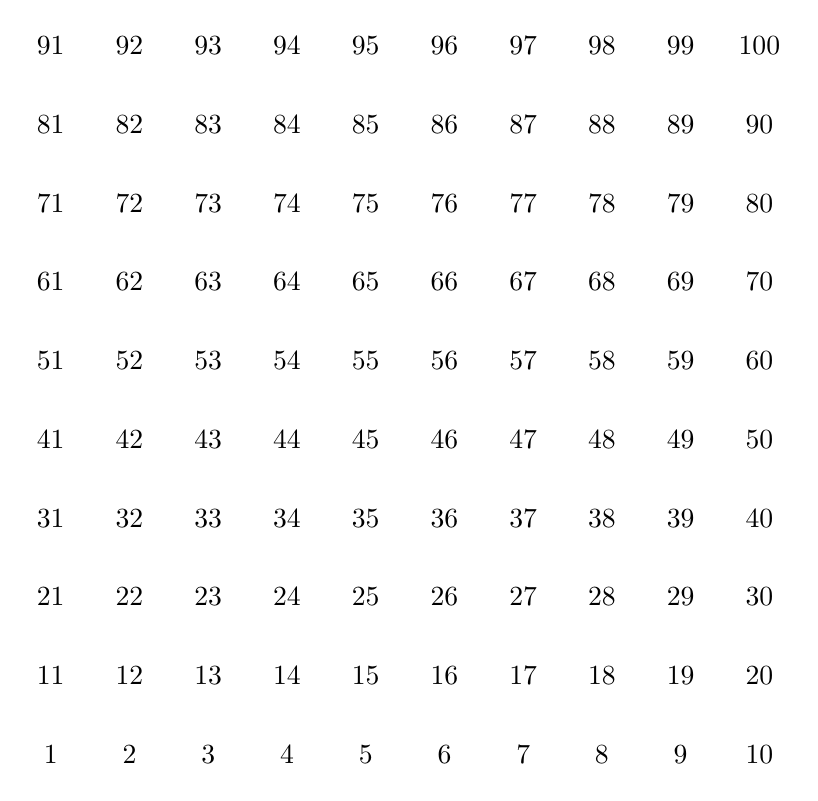
\begin{tikzpicture}[x=1cm, y=1cm]
\foreach \n [evaluate={%
    \x=mod(\n-1,10); 
    \y=floor((\n-1)/10);
    \p=isprime(\n);
    \e=mod(\n,2)==0;
    \style=(\p || \n==2) ? "prime" : (\e ? "even" : "odd");}] in {1,...,100}
    \node [every number/.try, every \style\space number/.try, number \n/.try]
       at (\x,\y) {\n};
\end{tikzpicture}

\egroup

\section{The \tikzname Library math}

The library defines a simple mathematical language to define simple functions and perform sequences
of basic mathematical operations.

PGF and \tikzname both use the PGF mathematical engine which provides numerous commands for parsing expressions. 
Unfortunately the pgf math engine is somewhat cumbersome for long sequences of mathematical operations,
particularly when assigning values to multiple variables. The TikZ calc library provides some additional
“convenience” operations for doing calculations (particularly with coordinates), but this can only be used
inside TikZ path commands.

The math library provides a means to perform sequences of mathematical operations in a more ‘user
friendly’ manner than the pgf math engine. In addition, the coordinate calculations of the calc library can
be accessed (provided it is loaded). However as the math library uses the pgf math engine – which uses
pure TEX to perform all its calculations – it is subject to the same speed and accuracy limitations. It is
worth bearing this in mind, before trying to implement algorithms requiring intensive and highly accurate
computation. You can, of course use the fp or the fpu libraries to increase the accuracy (but not necessarily
the speed) of computations.

For most purposes, the features provided by this library are accessed using the following command:

\begin{docCommand}{tikzmath}{\marg{statements}}
This command process a series of hstatementsi which can represent assignments, function definitions,
conditional evaluation, and iterations. It provides, in effect, a miniature mathematical language to
perform basic mathematical operations. Perhaps the most important thing to remember is that every
statement should end with a semi-colon. This is likely to be the most common reason why the \docAuxCommand{tikzmath}
command fails.
\end{docCommand}

\begin{texexample}{}{}
\tikz[x=0.25cm,y=0.25cm,
  evaluate={
    int \i, \j;
    for \i in {0,...,10}{
      for \j in {0,...,10}{
        \a{\i,\j} = (\i+\j)*5;
      };
    };
  }
]
\foreach \i in {0,...,10}
\foreach \j in {0,...,10}
\fill [red!\a{\i,\j}!yellow] (\i,\j) rectangle ++(1, 1);
\end{texexample}

Tantau in the pgfmanual provides an example as to how to calculate Fibonacci numbers. This demonstrates the beauty of this library, providing the clearlness of the commands, providing a familiar interface to persons to programmers.

\begin{texexample}{Calculating Fibonacci Numbers}{}
\tikzmath{
   function fibonacci(\n) {
    if \n == 0 then {
      return 0;
    } else {
       return fibonacci2(\n, 0, 1);
    };
   };
   function fibonacci2(\n, \p, \q) {
   if \n == 1 then {
     return \q;
    } else {
        return fibonacci2(\n-1, \q, \p+\q);
    };
   };
   int \f, \i;
   for \i in {0,1,...,20}{
      \f = fibonacci(\i);
      print {\f, };
    };
}
\end{texexample}


\section*{Declaring Functions}

One of the best ways to introduce complicated calculations is the declaration of functions.

\begin{texexample}{Calculating Fibonacci Numbers}{}
\tikzmath{
  function product(\x,\y) {
    return \x*\y;
  };
  int \i, \i, \k;
  \i = 22;
  \j = 22;
  \k = product(\i, \j);
  print { $\i\times \j = \k$ };
}
\end{texexample}

Once the types are extended, the library can be used almost as good as Lua, Go or any C based 
languages.



\begin{texexample}{Calculating Fibonacci Numbers}{}
\newcounter{tmath}
\setcounter{tmath}{5}
\tikzmath{
  function product(\x,\y) {
    return \x*\y;
  };
  int \i, \i, \k;
  \i = \thetmath; %a scratch counter
  \j = 500;
  \k = product(\i, \j);
  print {The counter (tmath) is: \thetmath\par };
  print { $\i\times \j = \k$ };
}
\end{texexample}



As this library is short manipulating dimensions, requires taht we strip the point from
the dimension. This can be achieved by the use of the \latexe macro \docAuxCommand{strip@pt}.
In the following example we can calculate the actual lengths of the \enquote{left} and \enquote{right}
margin of a page. 

\begin{texexample}{Page statistics}{ex:pgstats}
\makeatletter
\hoffset0pt
   \checkoddpage
  \ifoddpage
    This is an odd page\par
  \else
    I am even\par  
  \fi 
  
\global\newskip\myskip

\tikzmath{
  function addd(\x,\y) {
    return \x*\y+2;
  };
  real \pwidth, \pcalcwidth, \phoffset, \pvoffset, \poddsidemargin, \evensidemargin,
       \pmarginparwidth, \pmarginparsep,
       \textwidth,  
       \pheight;
%       
  \pwidth  = \strip@pt\paperwidth;  %paper width
  \pheight = \strip@pt\paperheight;
  \phoffset = \strip@pt\hoffset;
  \poddsidemargin = \strip@pt\oddsidemargin;
  \pevensidemargin = \strip@pt\evensidemargin;
  \pmarginparwidth = \strip@pt\marginparwidth;
  \pmarginparsep = \strip@pt\marginparsep;
  \ptextwidth    = \strip@pt\textwidth;
  \pcalcwidth = (72.52*2) + \poddsidemargin + \ptextwidth + \evensidemargin;
%  
  print {paper width = \the\paperwidth \par
         paper calculated right margin (abs) =\pgfmathsetlength\myskip{(\paperwidth-\textwidth)/2-(0.25*72.2pt)}\the\myskip\global\myskip=\myskip\par  
         paper hoffset = \phoffset pt\par
         paper oddsidemargin = \poddsidemargin pt\par
         paper evensidemargin = \pevensidemargin pt\par
         page marginparwidth = \pmarginparwidth pt\par
         page marginparsep   = \pmarginparsep pt\par
         page textwidth      = \ptextwidth pt\par
   };
}


\makeatother
\noindent\tikz[remember picture, overlay, outer sep=0pt,<->=Latex] \draw (\textwidth,0) -- ++(\myskip, 0)node {\the\myskip};

\noindent\tikz[remember picture, overlay, outer sep=0pt,<->=Latex] \draw (0,0) -- ++(-\myskip, 0);
\medskip
THIS \marginpar{{\tiny\lorem}}
\end{texexample}
  

       
% \even side margin
\noindent\tikz[remember picture, overlay, outer sep=2pt,<->, label=B]\draw[circle] (-\marginparsep-\marginparwidth-\evensidemargin,0) node{} -- ++(\evensidemargin, 0) node[label={right:\scriptsize\textbackslash evensidemargin}] {};
\medskip

% margin par
\noindent\tikz[remember picture, overlay, outer sep=2pt,<->]\draw (-\marginparsep,0) node[label=right:\scriptsize\textbackslash marginpar,outer sep=0pt]{} -- ++(-\marginparwidth, 0) node {};

% marginparsep

\noindent\tikz[remember picture, overlay, outer sep=2pt, <->] \draw (0,0)--(-\marginparsep,0) node[label=right:marginparsep]{};

\medskip

The textwidth can then be determined from the ratio of the outer margins.
% textwidth

\noindent\tikz[remember picture, overlay, outer sep=2pt,->]\draw (0,0) node{} -- ++(\the\textwidth, 0) node[label={\scriptsize \textbackslash textwidth}] {};

% draw at right
\noindent\tikz[remember picture, overlay, outer sep=2pt,->]\draw (\textwidth,0) node{} -- ++(\marginparsep, 0) node[label=right:{\scriptsize \textbackslash marginparsep}] {};

\noindent\tikz[remember picture, overlay, outer sep=2pt,->]\draw (\textwidth+\marginparsep,0) node{} -- ++(\marginparsep+\marginparwidth, 0) node[label=right:{\scriptsize \textbackslash marginparsep}] {};

% draw oddside margin
\medskip

Drawing the right margin

\tikzset{placeleft/.style = {outer sep=0pt, inner sep=0pt,label=left:{\scriptsize \textbackslash right margin}} }

\noindent\tikz[remember picture, overlay, outer sep=0pt,<->=Latex] \draw (\textwidth,0) -- ++(\myskip, 0)node {\the\myskip};

\noindent\tikz[remember picture, overlay, outer sep=0pt,<->=Latex] \draw (0,0) -- ++(-\myskip, 0);
\medskip


\lipsum[2]

\newpage
% \odd side margin
\noindent\tikz[remember picture, overlay, outer sep=2pt,<->, label=B]\draw[circle] (0,0) node{} -- ++(-\oddsidemargin-\evensidemargin, 0) node[label={right:\scriptsize\textbackslash oddsidemargin}] {};
\medskip

\lorem

% margin par
\noindent\tikz[remember picture, overlay, outer sep=2pt,<->]\draw (-\marginparsep,0) node[label=right:\scriptsize\textbackslash marginpar,outer sep=0pt]{} -- ++(-\marginparwidth, 0) node {};

% marginparsep

\noindent\tikz[remember picture, overlay, outer sep=2pt, <->] \draw (0,0)--(-\marginparsep,0) node[label=right:marginparsep]{};

\medskip

The textwidth can then be determined from the ratio of the outer margins.
% textwidth

\noindent\tikz[remember picture, overlay, outer sep=2pt,->]\draw (0,0) node{} -- ++(\the\textwidth, 0) node[label={\scriptsize \textbackslash textwidth}] {};

% draw at right
\noindent\tikz[remember picture, overlay, outer sep=2pt,->]\draw (\textwidth,0) node{} -- ++(\marginparsep, 0) node[label=right:{\scriptsize \textbackslash marginparsep}] {};

\noindent\tikz[remember picture, overlay, outer sep=2pt,->]\draw (\textwidth+\marginparsep,0) node{} -- ++(\marginparsep+\marginparwidth, 0) node[label=right:{\scriptsize \textbackslash marginparsep}] {};

% draw oddside margin
\noindent\tikz[remember picture, overlay, outer sep=0pt,<->=latex]\draw (\textwidth,0) node[placeleft]{} -- ++(120pt, 0) node{};

THIS \marginpar{{\tiny\lorem}}

\lipsum[2]

\newpage

\cxset{chapter format = lingerie, 
       %chapter aboveskip=30pt,
       chapter opening = any}



\newcommand\lingerie[2]{

\noindent
\tikzset{rules/.style = {color=white, top color = teal!70, bottom color=teal!50, line width=3pt} }
\vspace*{30pt}
\begin{tikzpicture}[remember picture, overlay, outer sep=0pt]
\draw[rules] (-10pt,0)--++(0, 1cm);
\draw[rules, line width=0.4pt] (-10pt-1.5pt,0) -- ++(\linewidth+3pt,0);
\draw[rules, line width=0.4pt] (-10pt-1.5pt,-2pt)-- ++(\linewidth+3pt,0);
\draw[rules] (-10pt,0) -- ++(0, -0.3\textheight);
\draw (0,0) node[above right, baseline=X.base] {\strut\upshape\LARGE\calligra #2};
\end{tikzpicture}

{\Large \color{black!70}
\parindent=0pt
\hsize=0.8\linewidth \raggedright
{M}{uch} boudoir photography is done on location. Whether it is your own home, your
model’s home, or a hotel in another city, shooting in different locations not only
provides variety but also allows you to offer different styles and themes.\par }
\vspace*{30pt}
}




\chapter{Lingerie}
\thispagestyle{empty}

\begin{multicols}{2}
\dropcap{A}{sking your client} to prepare her own hair and makeup can
mean less time for you on location but more time in postproduction.
A professional stylist can make a client look glamorous,
and usually have access to more dramatic makeup, fake lashes, and hair
extensions to give the client a more sultry look. Professionals will also
be skilled in covering imperfections that may be more visible with
regular makeup application. Better makeup means better shots
in-camera and less time in post-production. A professional makeup
artist has an artistic eye and knows exactly what colors and techniques
are needed to enhance the client’s best features. A good makeup artist
will also assess the wardrobe for the shoot to determine how bold or
creative the client’s look should be.

\lorem\lorem\lorem
\columnbreak
{
\parindent0pt

\includegraphics[width=\linewidth]{lingerie-02}
\par

}
\end{multicols}

\chapter{Wardrobe}
\thispagestyle{empty}
\begin{multicols}{2}
\lorem\lorem\lorem\lorem
Shadow edges in soft light can be so smooth that they disappear
altogether. The result is a less pronounced structure, which can hide
imperfections, but also a relatively low three-dimensionality. The
emphasis on bright, highly exposed or dark, lowly exposed parts in an
image can give photos a very strong expression. Images with mostly
bright areas are called high-key; images with mostly dark sections
low-key. This can be achieved either by having predominantly light- or
dark-colored elements in the picture, or by deliberately over- or
underexposing. Look at advertisements and movies and you will see
that this technique is widely used. 

\noindent\includegraphics[width=\columnwidth]{lingerie-01}\par

Write a caption on the other side if possible. Number your words.
\lorem\lorem
\end{multicols}

\newpage

\tikz[remember picture, overlay] \node[above right,xshift=-0.3cm, yshift=0.01cm] at (current page.south west){\includegraphics[height=1.0\paperheight]{lingerie-08}}; 

\chapter{Studio Lighting}
\thispagestyle{empty}
\begin{multicols}{2}
Studio lights help you light your subject in endless
different ways. You gain control by choosing the right lights for a
given job and become more independent from conditions that could
make your work difficult or even impossible.
The two main categories are continuous lights and flash. When you
work with continuous lights you need to watch your exposures just as
when working in daylight. Motion blur and camera shake are a danger
when shooting with slow shutter speeds. The current generation of
DSLRs perform very well at high ISO settings and help you keep
sufficient shutter speeds, even when light levels are low.
\end{multicols}

\tikz[remember picture, overlay] \node[above right,xshift=-0.3cm, yshift=-1cm] at (current page.south west){\includegraphics[width=1.05\paperwidth]{lingerie-06}}; %03

%\pagecolor{black!50}\color{white}
\chapter{Black and White}
\thispagestyle{empty}
\tikz[remember picture, overlay] \node[above right ,xshift=-0.3cm, yshift=-1cm] at (current page.south west){\includegraphics[width=1.05\paperwidth]{lingerie-07}}; %03

\newpage
test page



\newpage

%% Double Page spread with text
\thispagestyle{empty}

\tikz[remember picture, overlay] \node[below right,xshift=-0.2cm, yshift=0.2cm] at (current page.north west){\includegraphics[width=1.5\paperwidth]{korea-01}}; 

\newpage
\thispagestyle{empty}
\tikz[remember picture, overlay] \node[below left,xshift=-0.5\paperwidth+0.2cm, yshift=0.2cm] at (current page.north east){\includegraphics[width=1.5\paperwidth]{korea-01}};

\bgroup
\leftskip3.5in

The output routines possible with \tex are inadequate for books that have a modern style. Should we be able to measure the text and prohibit certain regions of the page from allowing text, i.e. only allow images, then everything is possible with minimum effort. \lipsum[1] \thepage
\egroup

\newpage

% reflect for better composition
\noindent\tikz[remember picture, overlay] \node[above right,xshift=-0.15cm, yshift=0.0cm] at (current page.south west) {
      \reflectbox{\includegraphics[height=1.01\paperheight]{balthus-01}}};


\chapter{The Full Page Pictures}

\begin{multicols}{2}
These are more difficult to achieve, firstly as we need to ensure that the pages do not contain any floats, which we need to flush before we typeset them.

Mark-up for such pages, bothered me for a while. It has to be as simple as possible, but at the same time as flexible as possible. We also face problems of rounding off that now and then the edges have small white spaces.

The aspect ratio of the page and the picture must be the same. We need to measure the image, which is not difficult.
\end{multicols}


\def\balthus#1{\newpage
 \pagecolor{creamy} 
 \checkoddpage
 \ifoddpage
  \tikz[remember picture, overlay] \node[above right,xshift=0.0cm, yshift=0.0cm, inner sep=0pt] at (current page.south west)    {\includegraphics[height=1.02\paperheight]{#1}};
  \else
  \tikz[remember picture, overlay] \node[above left,xshift=0.0cm, yshift=0.0cm, inner sep=0pt] at (current page.south east)  {\includegraphics[height=1.02\paperheight]{#1}};
 \fi
} 

\def\balthusin#1{\newpage
\thispagestyle{empty}
\parindent=0pt
 \pagecolor{white} 
 \checkoddpage
 \ifoddpage
  %\includegraphics[width=1.02\linewidth]{#1}\par
  \tikz \node[below right,xshift=0.0cm, yshift=0.0cm, inner sep=0pt, baseline=X.base] at (0,0)  {\includegraphics[width=1.02\linewidth]{#1}};\par
  \noindent\tikz[remember picture, overlay] \node[below right, baseline=X.base, inner sep=0pt] at (0.67\textwidth+7pt,\topskip-7pt){\parbox{4.4cm}{\scriptsize\smalllorem 1}};
  \else
  \tikz \node[below right,xshift=0.0cm, yshift=0.0cm, inner sep=0pt] at (0,0)  {\includegraphics[width=1.02\linewidth]{#1}};\par
  \tikz[remember picture, overlay] \node[below right, baseline=X.base] at (0.67\textwidth+7pt,\topskip){\lorem 2};
 \fi
} 


\balthus{balthus-02}

\balthus{balthus-03}

\balthus{balthus-05}

\balthus{balthus-04}

\balthus{balthus-06}

\balthusin{balthus-06}

\balthusin{balthus-07}
\bgroup
\small
\vfill\vfill
\vbox{\centering
\textit{\textbf{The Guitar Lesson}}, 1934\\
Oil on canvas, 161 x 138.5cm\\
Private collection\par\clubpenalty=10000}
\vfill
\egroup

\balthusin{balthus-08}
\bgroup
\hsize=.67\textwidth
\let\marginnotetextwidth\hsize
\lorem\lorem  A marginnote\marginnote{\scriptsize This is a margin note using the marginnote package} \lorem
\egroup

\balthusin{balthus-06}
\begin{multicols}{2}
\lorem
\end{multicols}
\end{document}